\chapter{Results}\label{sec:Chapter4-Results}

In this chapter, the proposed experiments are presented and explained. For each experiment, the results are shown and discussed.
There is a total of five proposed experiments:
\begin{itemize}[itemsep=0.1cm]
    \item \textbf{Experiment 1 - Preliminary Experiment:} aims to demonstrate the necessity of Hyperparameter Optimization (HPO) and to familiarize with the concepts of HPO.
    \item \textbf{Experiment 2 - Comparison of Optuna's Samplers on MNIST:} aims to evaluate the performance of different Hyperparameter Optimization algorithms, specifically Optuna's Samplers, on the MNIST dataset.
    \item \textbf{Experiment 3 - Comparison between a Custom PSO implementation and Optuna:} aims to compare the performance of a custom implementation of Particle Swarm Optimization (PSO) with Optuna's Samplers, on the MNIST dataset.
    \item \textbf{Experiment 4 - Comparison between a PSO Sampler and Optuna's Samplers:} aims to compare the performance of a PSO Sampler (made using Optuna as a base) with the other Optuna's Samplers, on the MNIST dataset.
    \item \textbf{Experiment 5 - Hyperparameter Optimization on Weed Map Dataset:} aims to perform Hyperparameter Optimization on the Weed Map Dataset, using Optuna.
\end{itemize}

\myparagraph{Experiments Source Code:}
All the source code of the experiments is available on the same repository \cite{Repository-THESIS} mentioned in the previous chapter (Chapter~\ref{sec:Chapter3-Methodology}), specifically in the \texttt{/experiments/} package.
In particular, the Weed Map Experiment (Experiment 5) is in the file \newline\texttt{/weed\_mapping\_experiment/Weed\_Mapping\_Optimization.ipynb}, while the other experiments were run using \texttt{/MNIST\_experiment/MNIST\_Optimization.ipynb}.

\section{Experiment 1 - Preliminary Experiment}

This Preliminary Experiment has a double goal.
The first is to familiarize with the concepts of HPO from a physical implementation perspective.
The second reason is to establish, if ever needed, the necessity of Hyperparameter Optimization; to demonstrate that HPO can actually improve the final performance of a ML experiment by finding the best Hyperparameters to train the model subject of the experiment with.
\\[0.3cm]Note that in this preliminary experiment, everything was developed with simple vanilla Python, without the use of the infrastructure described in the previous chapter (Chapter~\ref{sec:Chapter3-Methodology}).

\myparagraph{Hardware used for the Experiment:}
The hardware that was utilized to run this experiment is the following:
\begin{itemize}[itemsep=0.1cm]
    \item CPU: Intel Core i5-8265U CPU @ 1.60GHz (4-core, 8 thread)
    \item GPU: NVIDIA GeForce MX 110 (2GB VRAM)
    \item RAM: 8GB (DDR4)
    \item Disk: SSD
    \item OS: Windows 11
\end{itemize}

\subsection{Preparation of the Experiment}

Given the first goal of the experiment, the idea is to realize a simple implementation of the most traditional of HPO algorithms, which is Grid Search.
\\[0.3cm]The first part of the experiment consists in recreating another ML experiment which does not apply HPO and evaluating its results. Successively, the hyperparameters of that same ML model will be optimized with the custom Grid Search.
\\[0.3cm]The experiment chosen for comparison is the one proposed by the book “Dive Into Deep Learning” \cite{Tesi-1.6} (chapter 4 of the book). Some modifications have been made to this experiment: a simpler version of the proposed dataset is used; the Multi-Layer Perceptron (MLP) considered is implemented with vanilla Python rather than PyTorch.

\subsubsection{Dataset of the Experiment:}
The Dataset considered for the experiment is a simplified version of MNIST, specifically, the version included in scikit-learn \cite{scikit-learn}, from the function \texttt{load\_digits()} of the \texttt{dataset} module. (An explanation of the complete MNIST dataset is in the next experiment; for this preliminary experiment it is not necessary to understand the dataset).

\subsubsection{Model and Hyperparameters of the Experiment:}
As introduced earlier, the MLP model utilized is not the same as the one from the book. This is not detrimental to the scientific value of the experiment, as the considered hyperparameters and configuration of the model were the same as those proposed in the book, so that a comparison would still be possible.

\subsubsection{Implementation of Grid Search:}
The proposed implementation of Grid Search is completely made from scratch.
The algorithm takes as input the model, the dataset, and the grid of hyperparameters; the grid is a map object, where the keys are strings that represent the name of the hyperparameter, and the values are lists which contain the values that the corresponding hyperparameter can be.
\\[0.3cm]At the start of the algorithm, a Cartesian Product is applied to the lists inside the \texttt{param\_grid}, basically generating all the trials that are going to be evaluated.
For each trial, the model is initialized with the hyperparameters of that trial and evaluated; the results are saved in a variable.
After having completed all the trials, the algorithm returns as output the variable containing all the results, from which the best trial can be obtained.
\\[0.3cm]Two versions of this algorithm have been developed, one without parallelism and one with parallelism. There is no difference between the two, the only one is that the second allows to execute multiple trials on multiple threads.

\subsection{Execution of the Experiment}

The execution of the experiment is divided into three short parts: run and evaluation without hyperparameter optimization; run and evaluation with hyperparameter optimization; comparison of results.
\\[0.3cm]The set of hyperparameter utilized by the book for the experiment are the following (Tab.~\ref{tab:table-4.1.1}).
\begin{table}[ht!]
	\center
	\setlength{\tabcolsep}{0.5cm}
	\caption[Initial Hyperparameters of Experiment 1]{Initial hyperparameters of Experiment 1, as proposed by the book.}
	\begin{tabular}{@{}lc@{}}
		\toprule
		\textbf{Hyperparamter} & \textbf{Value} \\ \midrule
		Activation Input       & Sigmoid               \\[0.1cm]
		Activation Output      & Softmax               \\[0.1cm]
		Batch Size             & 256                   \\[0.1cm]
		Learning Rate          & 0.1                   \\[0.1cm]
		Hidden Size            & 10                    \\[0.1cm]
		Epochs                 & 10000                 \\ \bottomrule
	\end{tabular}
	\label{tab:table-4.1.1}
\end{table}
Training and evaluating the model with these hyperparameters lead to results of 99\% accuracy on the Training Set and 97\% on the Test Set.
The custom Grid Search algorithm is executed with the \texttt{param\_grid} in the figure (Fig.~\ref{fig:figure-4.1.1}) as input.
\begin{figure}[t]
	\centering
	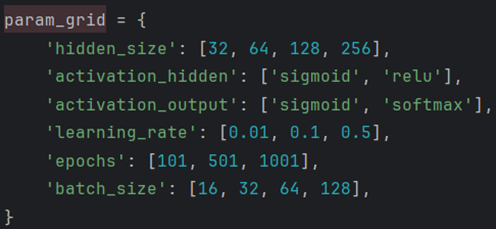
\includegraphics[width=8cm]{figures/figure-4.1.1.png}
	\caption[Param Grid for Custom Grid Search Experiment]{The Param Grid utilized for the Custom Grid Search Experiment.}
	\label{fig:figure-4.1.1}
\end{figure}
\\[0.3cm]The Grid Search algorithm executed a total of 576 trials. After the completion of the Optimization, there are three best results (with the same accuracy), which are in the figure (Fig.~\ref{fig:figure-4.1.2}).
\begin{figure}[b]
	\centering
	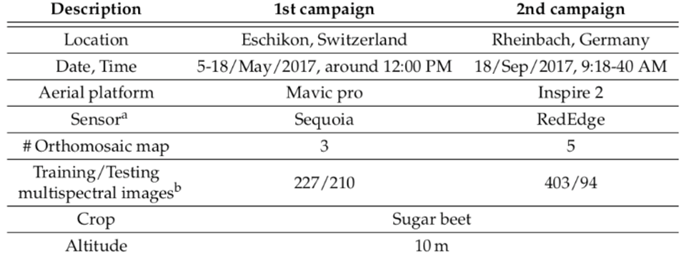
\includegraphics[width=15cm]{figures/figure-4.1.2.png}
	\caption[Best Results of Custom Grid Search Experiment]{The three best results of the Custom Grid Search Experiment.}
	\label{fig:figure-4.1.2}
\end{figure}
\\[0.3cm]These best results have an accuracy of 100\% on the Training Set and 98.6\% on the Test Set. Moreover, there are more than 20 trials with better accuracy than the configuration proposed by the book.

\subsection{Discussion of the Results}

This simple experiment with its results outlines how hyperparameter optimization, even when using a simple implementation of the weakest algorithm, could lead to a significant improvement in the performance of the trained model.
\\[0.3cm]The gained 1.6\% accuracy on the Test Set may seem like a little improvement, but is remarkable, especially when the dataset is composed of a very large number of observations.
\\[0.3cm]These results, additionally, confirm another aspect of HPO, which is the ability to improve the performance of an experiment without interfering with the model or the dataset.

\section{Experiment 2 - Comparison of Optuna's Samplers on MNIST}\label{sec:Experiment2-4.2}

The objective of this experiment is to evaluate the performance of different Hyperparameter Optimization algorithms so as to gain general knowledge about the capacity of each in preparation for subsequent, more complex experiments.
\\[0.3cm]In order to make the results and the methodology as much scientifically comparable as possible, rather than implementing various Samplers from scratch individually, a library for HPO is used.
\\[0.3cm]The chosen library is Optuna, which, as described in previous sections, includes a few Samplers already implemented, with the same style and same preconditions, making each optimization perfectly comparable to one another.
\\[0.3cm]As the idea is to have results that are as much general as possible, and because such “optimization of optimizations” is inevitably enormously expensive, a simple dataset is considered, which is MNIST.

\myparagraph{Hardware used for the Experiment:}
The hardware that was utilized to run this experiment is the following:
\begin{itemize}[itemsep=0.1cm]
	\item CPU: Intel Core i7-10700K CPU @ 3.80GHz
	\item GPU: NVIDIA GeForce RTX 3080 (10GB VRAM)
	\item RAM: 16GB (DDR5)
	\item Disk: SSD
	\item OS: Linux (Ubuntu)
\end{itemize}

\subsection{MNIST Dataset}

The MNIST Dataset is a database of images of handwritten digits \cite{MNIST}.
MNIST is the ideal dataset for learners and for small experiments regarding the field of pattern recognition, is basically a benchmarking dataset for Image Classification.
\\[0.3cm]Each image of the MNIST Dataset represents a digit from 0 to 9, making it ideal for benchmarking simple classification models for images (Fig.~\ref{fig:figure-4.1.3}).
\begin{figure}[t]
	\centering
	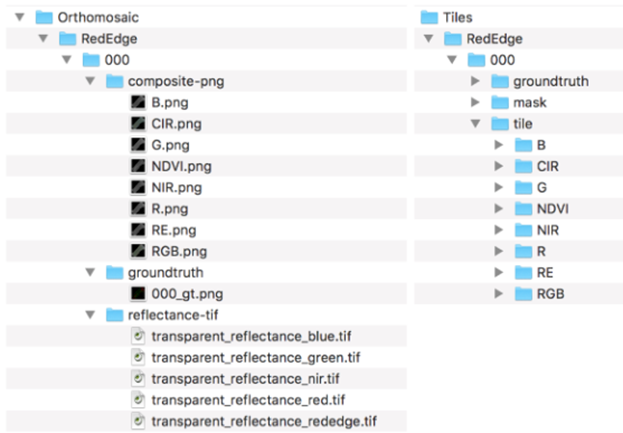
\includegraphics[width=9cm]{figures/figure-4.1.3.png}
	\caption[Examples of MNIST Images]{Some examples of images in the original MNIST dataset. Source:~\cite{MNIST}}
	\label{fig:figure-4.1.3}
\end{figure}

\subsubsection{Structure of MNIST Dataset}

The MNIST Dataset is composed of a total of 70000 images, of which 60000 are part of the training set and 10000 are part of the test set \cite{MNIST}.
The total weight of MNIST is 11.6MB when compressed, 52.3MB normally. Each image is 28x28 pixels, is in black and white, and weighs 784 bytes.

\myparagraph{NIST Dataset:}
MNIST is a newer version of an old dataset called NIST, in which the division was between SD-1 (Special Database 1) and SD-3 (Special Database 3); where SD-3 was the training set, and SD-1 the test set. The images of SD-3 were much clearer and easier to recognize.
\\[0.3cm]MNIST is designed so that half of its training images and half of its test images come from SD-1 and the remaining half from SD-3.
This means that half of the images of MNIST are easier to recognize, the other half are more difficult.

\subsubsection{Variants of MNIST Dataset}
Given its extreme simplicity to both use and understand, MNIST has inspired numerous variants. Some of the most famous variants are the following:
\begin{itemize}[itemsep=0.1cm]
    \item \textbf{Fashion-MNIST:} replaces digits with images of clothing items to test models on more complex visual patterns (Fig.~\ref{fig:figure-4.1.4}).
    \begin{figure}[t]
		\centering
		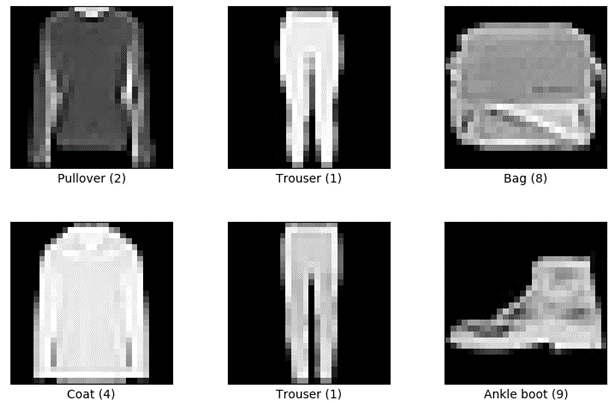
\includegraphics[width=10cm]{figures/figure-4.1.4.png}
		\caption[Examples of Fashion-MNIST Images]{Some examples of images in the Fashion-MNIST dataset. Source: Google Images}
		\label{fig:figure-4.1.4}
	\end{figure}
	\item \textbf{EMNIST (Extended MNIST):} includes, in addition to digits, also letters, to enhance the diversity of the dataset.
    \item \textbf{KMNIST:} includes images of Japanese Kanji characters, making the classification task much more complex than the version on the Latin alphabet.
    \item \textbf{NoiseMNIST:} is a version of MNIST where Gaussian noise is added to the images, it is useful to test the robustness of the model against noisy data.
    \item \textbf{Rotated MNIST:} is a version of MNIST where the images are rotated by a random angle, to test the robustness of the model against rotated data.
\end{itemize}
% 
% \myparagraph{Fashion-MNIST:}
% Fashion-MNIST replaces digits with images of clothing items to test models on more complex visual patterns.
% \begin{figure}[t]
% 	\centering
% 	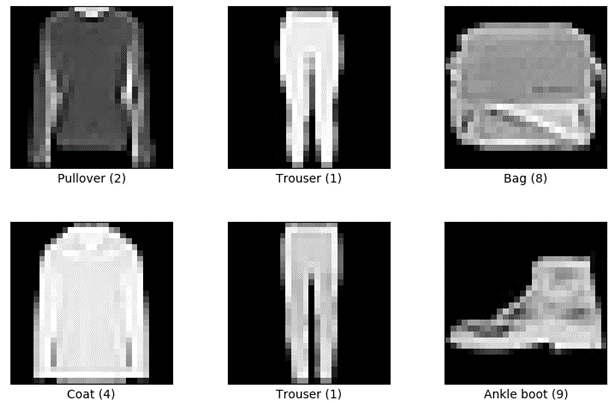
\includegraphics[width=15cm]{figures/figure-4.1.4.png}
% 	\caption[Examples of Fashion-MNIST Images]{Some examples of images in the Fashion-MNIST dataset. Source: Google Images}
% 	\label{fig:figure-4.1.4}
% \end{figure}
% 
% \myparagraph{EMNIST (Extended MNIST):}
% EMNIST includes, in addition to digits, also letters, to enhance the diversity of the dataset.
% 
% \myparagraph{KMNIST:}
% KMNIST includes images of Japanese Kanji characters, making the classification task much more complex than the version on the Latin alphabet.
% 
% \myparagraph{NoiseMNIST:}
% NoiseMNIST is a version on MNIST where Gaussian noise is added to the images, it is useful to test the robustness of the model against noisy data.

\subsection{Preparation of the Experiment}

The preparation for the experiment is simple: using the code infrastructure described in the Methodology chapter, specifically the section on Optuna Enhancing (Sec.~\ref{sec:EnhancingOptuna-3.3}), an Optuna's \texttt{Study} object is created and run.
\\[0.3cm]The MNIST dataset was imported through the \texttt{MNIST} package of Pytorch, included in torchvision, and then loaded with PyTorch data loaders.

\subsubsection{Setup of the Studies}

% \myparagraph{Initialize the Studies:}
The Samplers of Optuna subject of this experiment are the following: \texttt{RandomSampler}, \texttt{TPESampler}, \texttt{CmaEsSampler}, \texttt{GPSampler}, \texttt{NSGAIISampler}, \texttt{PartiallyFixedSampler}, \texttt{QMCSampler}.
For each of the Samplers, an Optuna \texttt{Study} is created. All the samplers are initialized with their default input values.
\\[0.3cm]The Pruner utilized for each Study is the Hyperband (\texttt{HyperbandPruner} object in Optuna), initialized with its default input values.

\subsubsection{Setup of the Objective Function}

% \myparagraph{Objective Function:}
The objective function, obviously the same for each Study, is divided into three sections: Declaration of the Hyperparameters to optimize and their value ranges; Initialization of the model and related objects; Training and Evaluation of the model.
\\[0.3cm]At the execution of each trial, for each hyperparameter, a value is sampled by Optuna's Sampler, then those values are used to initialize the model and its related objects, training included, and the training loop can start. The value then returned will be the score.
% 
% \myparagraph{Search Space of Hyperparameters:}
\\[0.3cm]The Hyperparameters declared in the objective function, which form the Search Space of the Study, for this experiment were the following (Tab.~\ref{tab:table-4.2.1}).
\begin{table}[ht!]
	\center
	\setlength{\tabcolsep}{0.5cm}
	\caption[Search Space of Experiment 2]{Search Space of Experiment 2: list of hyperparameters and their values ranges, with the step. Where Step is $\sim$ if the range is continuous.}
	\begin{tabular}{@{}lcc@{}}
		\toprule
		\textbf{Hyperparamter}   & \textbf{Range}             & \textbf{Step} \\ \midrule
		Activation Function      & \{ReLU, tanh, sigmoid\}    & -             \\[0.1cm]
		Batch Size               & {[}16, 64{]}               & 16            \\[0.1cm]
		Epochs                   & 10                         & -             \\[0.1cm]
		Hidden Layer Width \{i\} & {[}8, 128{]}               & 8             \\[0.1cm]
		Hidden Layer Depth       & {[}1, 3{]}                 & 1             \\[0.1cm]
		Learning Rate            & {[}$10^{-5}$, $10^{-1}${]} & $\sim$        \\[0.1cm]
		Loss Function            & \{CrossEntropy, Focal\}    & -             \\[0.1cm]
		Optimizer                & \{SGD, Adam\}              & -             \\ \bottomrule
	\end{tabular}
	\label{tab:table-4.2.1}
\end{table}
% 
% \myparagraph{Optimizing Process Parameters:}
\\[0.3cm]Other parameters, related to the Optimization process, basically hyperparameters of the HPO process itself (could be called “Hyper-Hyperparamters”), which were used are the following (Tab.~\ref{tab:table-4.2.2}).
\begin{table}[ht!]
	\center
	\setlength{\tabcolsep}{0.5cm}
	\caption[Optimization External Parameters of Experiment 2]{External optimization parameters of Experiment 2, basically hyperparameters of the optimization process, with their values.}
	\begin{tabular}{@{}llc@{}}
		\toprule
		\textbf{Group} & \textbf{Parameter} & \textbf{Value} \\ \midrule
		Regularizer    & labda              & 0.4            \\[0.1cm]
		EarlyStopper   & patience           & 5              \\ \bottomrule
	\end{tabular}
	\label{tab:table-4.2.2}
\end{table}

\subsection{Execution of the Experiment}

The execution of each Study is handled by an \texttt{OptunaRunner} object, which at the end of the optimization process saves the results on a csv file.
\\[0.3cm]The number of Trials executed for each Study was 128.
\\[0.3cm]In the reporting of the results, the information regarding what the best hyperparameters' values are will be ignored, because it is not the focus of the experiment, which is to identify how well performing the various techniques are.
\\[0.3cm]For the experiment, each Study has been executed around six times (some had more executions than others); the reported results are therefore a mean of the multiple results from the multiple executions. 

\subsubsection{RandomSampler}

The best score achieved by the \texttt{RandomSampler} is 91.7\%; there are 29 trials with a score over 80\% and 3 with a score over 90\%. The Accuracy of these top trials is around 95\%-97\%.
\\[0.3cm]In terms of Accuracy, the best score is 98\% and the best results are around 97\%, but those results have lower regularized scores.
\\[0.3cm]The results of the \texttt{RandomSampler} are useful to compare the results of the other samplers, to see if there is an actual advantage in using them for these experiments, or if they are just equivalent to the random approach.

\subsubsection{TPESampler}

The best score achieved by the \texttt{TPESampler} is 94\%, which is the best score of the whole experiment; there are 101 trials with a score over 80\%; 60 with a score over 90\%; 13 with a score over 93\%. The Accuracy of these top trials is around 94\%-96\%.
\\[0.3cm]In terms of Accuracy, the best scores are all close to 98\%, but all those best scores are also the worst in terms of regularized score.
\\[0.3cm]Talking about the network architectures, the best scores were achieved with a single hidden layer architecture, other good scores were achieved even with a linear architecture, or with a two-hidden-layer architecture where the total number of neurons was minimally higher than the single layer one.

\subsubsection{CmaEsSampler}

After a total of five tries, the execution of the studies never terminated without errors.
It is likely that the setup values of the experiment are not compatible with the default initialization values of this sampler.
Therefore, this Sampler will be discarded.

\subsubsection{GPSampler}

The best scores achieved by \texttt{GPSampler}, both in terms of Accuracy and in terms of regularized score, are basically equivalent to the results of \texttt{RandomSampler}.
In order to give more possibilities to the sampler, various initialization values were tried, none of which changed the results.
It is not completely clear why this sampler produces results equivalent to those of \texttt{RandomSampler}, this will be further discussed in the Discussion section.

\subsubsection{NSGAIISampler}

The best scores achieved by \texttt{NSGAIISampler}, both in terms of Accuracy and in terms of regularized score, are basically equivalent to the results of \texttt{RandomSampler}.
In order to give more possibilities to the sampler, various initialization values were tried, none of which changed the results.
It is not completely clear why this sampler produces results equivalent to those of \texttt{RandomSampler}, this will be further discussed in the Discussion section.

\subsubsection{PartiallyFixedSampler}

The \texttt{PartiallyFixedSampler} was failing in the first execution because, as the name suggests, it is a type of sampler that requires some hyperparameters of the defined Search Space to be fixed.
\\[0.3cm]The choice was not to further continue using this sampler, as the objective of the experiment is to evaluate the sampling technique rather than to actually find the best hyperparameters' values, or correlations in the Search Space.
Therefore, this Sampler will be discarded.

\subsubsection{QMCSampler}

The best scores achieved by \texttt{QMCSampler}, both in terms of Accuracy and in terms of regularized score, are basically equivalent to the results of \texttt{RandomSampler}.
In order to give more possibilities to the sampler, various initialization values were tried, none of which changed the results.
It is not completely clear why this sampler produces results equivalent to those of \texttt{RandomSampler}, this will be further discussed in the Discussion section.

\subsection{Discussion of the Results}

This experiment, with the execution of these studies, allowed to establish important ground knowledge about the efficacy of the most important sampling techniques of Hyperparameter Optimization.

\subsubsection{Analysis of the Best Hyperparameters Results}

For the record, even if it is not in the main objectives of the experiment, the best hyperparameters found by the most reliable Sampler (\texttt{TPESampler}) were the following (Tab.~\ref{tab:table-4.2.3}).
% \begin{itemize}[itemsep=0.1cm]
%     \item Activation = ReLU
%     \item Loss = CrossEntropy
%     \item Architecture = [input, 16, output]
%     \item Batch Size = 16
%     \item Optimizer = Adam
% \end{itemize}
\begin{table}[ht!]
	\center
	\setlength{\tabcolsep}{0.5cm}
	\caption[Best Hyperparameters of Experiment 2]{Best hyperparameters of Experiment 2, found by with the optimization process with \texttt{TPESampler}.}
	\begin{tabular}{@{}lc@{}}
		\toprule
		\textbf{Hyperparamter} & \textbf{Value}          \\ \midrule
		Activation             & ReLU                    \\[0.1cm]
		Loss                   & CrossEntropy            \\[0.1cm]
		Architecture           & {[}input, 16, output{]} \\[0.1cm]
		Batch Size             & 16                      \\[0.1cm]
		Optimizer              & Adam                    \\ \bottomrule
	\end{tabular}
	\label{tab:table-4.2.3}
\end{table}
It is vital to note that, given the simplicity of the dataset, in some executions, the best hyperparameters' values were different (except model architecture), outlining how in simple problems like this one, the only really impactful factor was the architecture of the NN, while the possible combinations of the other hyperparameters able to achieve high results were many.

\subsubsection{Analysis of the Failed Samplers}

With regard to the two failed sub-experiments, which are, the studies using respectively \texttt{CmaEsSampler} and \texttt{PartiallyFixedSampler}, for the sake of simplicity, these samplers will be discarded.
In order to conduct the next experiments, it was already necessary to identify the best samplers and discard the worst ones; so, discarding the failing samplers is the least time-consuming solution.

\subsubsection{Analysis of the Worst Performing Samplers}

As for the performance of \texttt{GPSampler}, \texttt{NSGAIISampler} and \texttt{QMCSampler}, one possible hypothesis for the reason their results are equivalent to \texttt{RandomSampler}, is the simplicity of the dataset and the model.
\\[0.3cm]The hypothesis is, given that, as mentioned above, there is only one impactful hyperparameter, it is unlikely for these more complex sampling algorithms to find correlations in the Search Space, making the search partially unsuccessful.
Therefore, for the next experiments, these three samplers will be discarded.

\subsubsection{Analysis of the Best Samplers}

The best results were obtained by the Study using \texttt{TPESampler}. The trend in the results suggests that the \texttt{TPESampler} is actually learning from past trials throughout the optimization process, as the best results are mostly in the later stages of the optimization.
\\[0.3cm]Therefore, with regard to the first objective of the experiment, it can be concluded that \texttt{TPESampler} can be used for the other experiments. Together with \texttt{TPESampler}, also \texttt{RandomSampler} can be used, because it did not show any unexpected behaviour and can thus be applied to make first assessments.
\\[0.3cm]In conclusion, now that the best performing samplers are well-established, in the next experiments they can be utilized as a tool of comparison with other new sampling techniques. 

\subsubsection{Analysis of the Best NN Architectures}

For what concerns the second objective of the experiment, which is to find lightweight, but well-performing nonetheless solutions, \texttt{TPESampler} gained interesting results.
\\[0.3cm]The theoretical hypothesis was that, at the same total number of neurons, deeper architectures would have reached better scores. The results suggest, however, that there is no difference between the two, sometimes even linear architectures have achieved a good score.
\\[0.3cm]From these results, it can be concluded that the experiment, and especially the model, are too simple for the score to be significantly different between deeper and less deep networks. Deeper networks do not result in an increase in generalization power if the model and the experiment are excessively simple.

\section{Experiment 3 - Comparison between a Custom PSO implementation and Optuna}

The goal of this experiment is to test and evaluate the functioning and performance of the custom implementation of Particle Swarm Optimization, adapted for HPO in a way that is similar to Optuna, and compare such performance to that of the samplers of Optuna.
\\[0.3cm]In order to make the results and the methodology as much scientifically comparable as possible, as described in the methodology chapter (Sec.~\ref{sec:CustomImplementationOfPSO-3.2}), the implementation of PSO replicates almost perfectly the functioning of Optuna and displays the result in the same exact way.
\\[0.3cm]As the goal of the experiment is primarily to compare a new technique to existent techniques, and therefore would be excessive to operate on a complex and expensive problem, a simple dataset is considered, which again is MNIST.

\myparagraph{Hardware used for the Experiment:}
The hardware that was utilized to run this experiment is the same as Experiment 2 (Sec.~\ref{sec:Experiment2-4.2}).

\subsection{Preparation of the Experiment}

The preparation for the experiment is similar to Experiment 2 (Sec.~\ref{sec:Experiment2-4.2}): the Studies related to the samplers of Optuna continue to be initialized with the “wrapping”, whereas the Study for the custom PSO is initialized separately. Nevertheless, the process is basically the same, given that it is supposed to be a sort of replica of Optuna. 
\\[0.3cm]The MNIST dataset was imported through the \texttt{MNIST} package of Pytorch, included in torchvision, and then loaded with PyTorch data loaders.

\subsubsection{Setup of the Studies}

% \myparagraph{Initialize the Studies:}
The Samplers of Optuna subject of this experiment are the following: \texttt{RandomSampler}, \texttt{TPESampler}.
For each of the Samplers, an Optuna \texttt{Study} is created. All the samplers are initialized with their default input values.
The Study of the custom PSO is called \texttt{PSO\_optimization}.
\\[0.3cm]As a result of the subsequent lack of scientific comparability between the two approaches if the pruning mechanism was involved for both, the Pruner is disabled.

\subsubsection{Setup of the Objective Function}

% \myparagraph{Objective Function:}
The objective function is the same for each Study, even for the \texttt{PSO\_optimization} Study. The structure of the objective function is the same as the last experiment.
% 
% \myparagraph{Search Space of Hyperparameters:}
\\[0.3cm]The Hyperparameters declared in the objective function, which form the Search Space of the Study, for this experiment were the following (Tab.~\ref{tab:table-4.3.1}).
\begin{table}[ht!]
	\center
	\setlength{\tabcolsep}{0.5cm}
	\caption[Search Space of Experiment 3]{Search Space of Experiment 3: list of hyperparameters and their values ranges, with the step. Where Step is $\sim$ if the range is continuous.}
	\begin{tabular}{@{}lcc@{}}
		\toprule
		\textbf{Hyperparamter} & \textbf{Range}             & \textbf{Step} \\ \midrule
		Activation Function    & \{ReLU, tanh, sigmoid\}    & -             \\[0.1cm]
		Hidden Layer Width 1   & {[}0, 128{]}               & 1             \\[0.1cm]
		Hidden Layer Width 2   & {[}0, 128{]}               & 1             \\[0.1cm]
		Hidden Layer Width 3   & {[}0, 128{]}               & 1             \\[0.1cm]
		Learning Rate          & {[}$10^{-4}$, $10^{-2}${]} & $\sim$        \\[0.1cm]
		Optimizer              & \{SGD, Adam\}              & -             \\ \bottomrule
	\end{tabular}
	\label{tab:table-4.3.1}
\end{table}
% 
% \myparagraph{Optimizing Process Parameters:}
\\[0.3cm]Other parameters, related to the Optimization process, basically hyperparameters of the HPO process itself (could be called “Hyper-Hyperparamters”), which were used are the following (Tab.~\ref{tab:table-4.3.2}).
\begin{table}[ht!]
	\center
	\setlength{\tabcolsep}{0.5cm}
	\caption[Optimization External Parameters of Experiment 3]{External optimization parameters of Experiment 3, basically hyperparameters of the optimization process, with their values.}
	\begin{tabular}{@{}llc@{}}
		\toprule
		\textbf{Group}               & \textbf{Parameter} & \textbf{Value} \\ \midrule
		Regularizer                  & labda              & 0.4            \\[0.1cm]
		EarlyStopper                 & patience           & 5              \\[0.2cm]
		\multirow{2}{*}{PSOStopping} & patience           & 5              \\[0.1cm]
									 & tolerance          & 0.005          \\[0.2cm]
		\multirow{2}{*}{PSO}         & num\_particles     & 32             \\[0.1cm]
									 & max\_generations   & 8              \\ \bottomrule
	\end{tabular}
	\label{tab:table-4.3.2}
\end{table}

\subsection{Execution of the Experiment}

The execution of each Study is handled by an \texttt{OptunaRunner} object for Optuna and by \texttt{PSORunner} for PSO (it is exactly the same); which, at the end of the optimization process, saves the results on a csv file.
\\[0.3cm]The number of Trials executed for each Study was 256.
\\[0.3cm]In the reporting of the results, the information regarding what the best hyperparameters' values are will be ignored, because it is not the focus of the experiment, which is to identify how well performing the various techniques are.

\subsubsection{RandomSampler}

The best score achieved by the \texttt{RandomSampler} is 92\%; there are 42 trials with a score over 80\% and 2 with a score over 90\%. The Accuracy of these top trials is around 95\%-97\%.
\\[0.3cm]In terms of Accuracy, the best score is 98\% and the best results are around 97\%, but these results have far lower regularized scores.
\\[0.3cm]As every experiment, these results from the \texttt{RandomSampler} have the purpose of evaluating how well the new techniques are performing, and whether they are doing what supposed to or are just collapsing into a random sampling.

\subsubsection{TPESampler}

The best score achieved by the \texttt{TPESampler} is 93.2\%, there are 224 trials with a score over 80\%; 135 with a score over 90\%; 5 with a score over 93\%. The Accuracy of these top trials is around 95\%-96\%.
\\[0.3cm]In terms of Accuracy, the best scores are all around 97\%, but these results have far lower regularized scores.

\subsubsection{PSO\_optimization}

The best score achieved by the custom PSO algorithm is 93\%, there are 123 trials with a score over 80\%; 22 with a score over 90\%; 2 with a score over 93\%. The Accuracy of these top trials is around 95\%-96\%.
\\[0.3cm]In terms of Accuracy, the best scores are all close to 98\%, but these results have far lower regularized scores.

\subsection{Discussion of the Results}

The results of the experiment allow to safely conclude that the proposed adaptation of PSO to HPO was successful and is also perfectly comparable with the results from the Studies of Optuna.

\subsubsection{Analysis on the Custom PSO Results}

The results presented by the \texttt{PSO\_optimization} Study, allow to establish that the algorithm is working as intended, the process is learning from past Trials.
Analysing the results, it appears evident that the best scores have been obtained at the latest generations, outlining how the Particles are correctly closing their distance with the global optimum over time.

\subsubsection{Analysis of the Comparison with Optuna}

After comparing the results from the \texttt{PSO\_optimization} Study, \texttt{RandomSampler} and \texttt{TPESampler}, it is easy to see that the PSO reaches similar levels of quality.
\\[0.3cm]The comparison with \texttt{RandomSampler} clearly shows that the PSO is not sampling randomly, but is following a logic, based on the PSO algorithm.
\\[0.3cm]The comparison with \texttt{TPESampler} allows to say that PSO is also extremely well-performing, and can be used in the same way as the TPESampler. The former has indeed found a greater number of very good solutions, but this is also because PSO has the tendency to never stop the exploration; in fact, watching the trial number around which the two algorithms started to find good solutions, it is almost the same; the main difference is a result of the characteristic of the TPE to focus on exploitation toward the last trials, which in this case led to slightly better results compared to PSO.

\section{Experiment 4 - Comparison between a PSO Sampler and Optuna's Samplers}

In the previous experiment, a custom implementation of PSO external to Optuna was tested, evaluated, and compared to the performance of Optuna.
\\[0.3cm]This experiment instead, aims to test, evaluate, and compare the \texttt{PSOSampler}, a Sampler developed within Optuna that implements the PSO algorithm, described in the Methodology chapter in the related section (Sec.~\ref{sec:CustomOptunaPSOSampler-3.3.2}).
\\[0.3cm]In this way, the results will already be perfectly comparable to the ones of the native samplers of Optuna. The same exact code infrastructure utilized for the Studies of Optuna, can also be used for the Study which uses the \texttt{PSOSampler}.
\\[0.3cm]The experiment is divided into two sub-experiments, with the same approach and the same goals. The only difference between the two is that in the first Pruning is disable, in the second is enabled.
\\[0.3cm]As the goal of the experiment is primarily to compare a new technique to existent techniques, and therefore would be excessive to operate on a complex and expensive problem, a simple dataset is considered, which again is MNIST.

\myparagraph{Hardware used for the Experiment:}
The hardware that was utilized to run this experiment is the same as Experiment 2 (Sec.~\ref{sec:Experiment2-4.2}).

\subsection{Preparation of the Experiment}

The preparation for the experiment is very similar to Experiment 2 (Sec.~\ref{sec:Experiment2-4.2}): now \texttt{PSOSampler} has become a Sampler of Optuna, thus initializing its related \texttt{Study} object is the same procedure as the standard Studies of Optuna; they continue to be initialized with the “wrapping”.
\\[0.3cm]The MNIST dataset was imported through the \texttt{MNIST} package of Pytorch, included in torchvision, and then loaded with PyTorch data loaders.

\subsubsection{Setup of the Studies}

% \myparagraph{Initialize the Studies:}
The samplers of Optuna subject of this experiment are the following: \texttt{RandomSampler}, \texttt{TPESampler}, \texttt{PSOSampler}.
For each of the samplers, an Optuna \texttt{Study} is created. All the standard samplers are initialized with their default input values. The \texttt{PSOSampler} is initialized with two values, \texttt{num\_particles} and \texttt{max\_generations}.
\\[0.3cm]For the experiment where Pruning is enabled, the Hyperband algorithm is used, applied through the \texttt{HyperbandPruner} object of Optuna.

\subsubsection{Setup of the Objective Function}

% \myparagraph{Objective Function:}
The objective function, as always, is the same for each Study. The structure of the objective function is the same as in the last experiments.
% 
% \myparagraph{Search Space of Hyperparameters:}
\\[0.3cm]The Hyperparameters declared in the objective function, which form the Search Space of the Study, for this experiment were the following (Tab.~\ref{tab:table-4.4.1}).
\begin{table}[ht!]
	\center
	\setlength{\tabcolsep}{0.5cm}
	\caption[Search Space of Experiment 4]{Search Space of Experiment 4: list of hyperparameters and their values ranges, with the step. Where Step is $\sim$ if the range is continuous.}
	\begin{tabular}{@{}lcc@{}}
		\toprule
		\textbf{Hyperparamter} & \textbf{Range}             & \textbf{Step} \\ \midrule
		Activation Function    & \{ReLU, tanh, sigmoid\}    & -             \\[0.1cm]
		Hidden Layer Width 1   & {[}0, 128{]}               & 8             \\[0.1cm]
		Hidden Layer Width 2   & {[}0, 128{]}               & 8             \\[0.1cm]
		Hidden Layer Width 3   & {[}0, 128{]}               & 8             \\[0.1cm]
		Learning Rate          & {[}$10^{-4}$, $10^{-2}${]} & $\sim$        \\[0.1cm]
		Optimizer              & \{SGD, Adam\}              & -             \\ \bottomrule
	\end{tabular}
	\label{tab:table-4.4.1}
\end{table}
% 
% \myparagraph{Optimizing Process Parameters:}
\\[0.3cm]Other parameters, related to the Optimization process, basically hyperparameters of the HPO process itself (could be called “Hyper-Hyperparamters”), which were used are the following (Tab.~\ref{tab:table-4.4.2}).
\begin{table}[ht!]
	\center
	\setlength{\tabcolsep}{0.5cm}
	\caption[Optimization External Parameters of Experiment 4]{External optimization parameters of Experiment 4, basically hyperparameters of the optimization process, with their values.}
	\begin{tabular}{@{}llc@{}}
		\toprule
		\textbf{Group}                   & \textbf{Parameter} & \textbf{Value} \\ \midrule
		Regularizer                      & labda              & 0.4            \\[0.1cm]
		EarlyStopper                     & patience           & 5              \\[0.2cm]
		\multirow{2}{*}{PSOSampler}      & num\_particles     & 32             \\[0.1cm]
										 & max\_generations   & 8              \\[0.2cm]
		\multirow{4}{*}{HyperbandPruner} & min\_resources     & 3              \\[0.1cm]
										 & max\_resources     & 30             \\[0.1cm]
										 & reduction\_factor  & 3              \\[0.1cm]
										 & bootstrap\_count   & 6              \\ \bottomrule
	\end{tabular}
	\label{tab:table-4.4.2}
\end{table}

\subsection{Execution of the Experiment}

The execution of each Study is handled by an \texttt{OptunaRunner} object for Optuna, which at the end of the optimization process saves the results on a csv file.
\\[0.3cm]The number of Trials executed for each Study was 256.
\\[0.3cm]In the reporting of the results, the information regarding what the best hyperparameters' values are will be ignored, because it is not the focus of the experiment, which is to identify how well performing the various techniques are.

\subsubsection{RandomSampler  vs  TPESampler  vs  PSOSampler  -  No Pruning}

The best score achieved by the \texttt{RandomSampler} is 92\%; there are 42 trials with a score over 80\% and 2 with a score over 90\%. The Accuracy of these top trials is around 95\%-97\%.
\\[0.3cm]The best score achieved by the \texttt{TPESampler} is 93.2\%; there are 224 trials with a score over 80\%; 135 with a score over 90\%; 5 with a score over 93\%. The Accuracy of these top trials is around 95\%-96\%.
\\[0.3cm]The best score achieved by the \texttt{PSOSampler} is 93.8\%; there are 174 trials with a score over 80\% and 117 with a score over 90\%. 28 with a score over 93\%. The Accuracy of these top trials is around 95\%-96\%.

\subsubsection{RandomSampler  vs  TPESampler  vs  PSOSampler  -  With Pruning}

The best score achieved by the \texttt{RandomSampler} is 90.6\%; there are 29 trials with a score over 80\% and 1 with a score over 90\%. The Accuracy of these top trials is around 91\%-97\%.
\\[0.3cm]The best score achieved by the \texttt{TPESampler} is 94\%; there are 216 trials with a score over 80\%; 105 with a score over 90\%; 41 with a score over 93\%. The Accuracy of these top trials is around 95\%-96.5\%.
\\[0.3cm]The best score achieved by the \texttt{PSOSampler} is 93.4\%; there are 156 trials with a score over 80\% and 89 with a score over 90\%. 9 with a score over 93\%. The Accuracy of these top trials is around 94\%-95\%.

\subsection{Discussion of the Results}

The results of the experiment, in the first place, demonstrated the validity of the \texttt{PSOSampler}, showing that it works as supposed and is perfectly integrated in Optuna, being executed without errors and reaching good results.
Another really positive outcome, is the confirmation of the applicability of PSO to Hyperparameter Optimization. This experiment further proved what was already being suggested by the previous one. 

\subsubsection{Analysis of the Results of PSOSampler}

The \texttt{PSOSampler} is clearly working as intended, and the implementation of a custom sampler within Optuna has been revealed to be successful.
The \texttt{PSOSampler}, as confirmed by the results, obtained top-level results; finding the best among possible candidate solutions for the given problem.

\subsubsection{Analysis of the Comparison with Optuna}

The results showed that \texttt{PSOSampler} can even outperform the most powerful Optuna's samplers, in fact, the \texttt{PSOSampler} had better results than the \texttt{TPESampler} in the sub-experiment without pruning.
In the other sub-experiment, the one with pruning, it reached slightly worse results than the \texttt{TPESampler}. Intuitively, it makes sense for a PSO algorithm to suffer pruning, because in order for its functioning to be as much accurate as possible, it needs all the information regarding the Search Space, and the concept of pruning remove some of that information.

\subsubsection{Analysis of the Trials Performance Distribution}

In order to show how the Samplers improve over time, a scatter plot can be used, with the Trial number on one axis and the score on the other.
\\[0.3cm]In the \texttt{RandomSampler} is evident how the search is searching randomly within the space, there is no learning from the past trials (Fig.~\ref{fig:figure-4.4.2}).
\\[0.3cm]In the \texttt{TPESampler} it can be observed how, even after relatively few trials, the score starts becoming better and better, learning from previous trials (Fig.~\ref{fig:figure-4.4.3}).
\\[0.3cm]In the \texttt{PSOSampler}, as in the \texttt{TPESampler}, the algorithm learns from the past trials. It can be seen how this “convergence” happens later compared to the \texttt{TPESampler}, this is because PSO is initially an explorative technique, that only in later generations starts to accumulate trials toward the best solution (Fig.~\ref{fig:figure-4.4.4}).
% \begin{figure}[t]
% 	\centering
% 	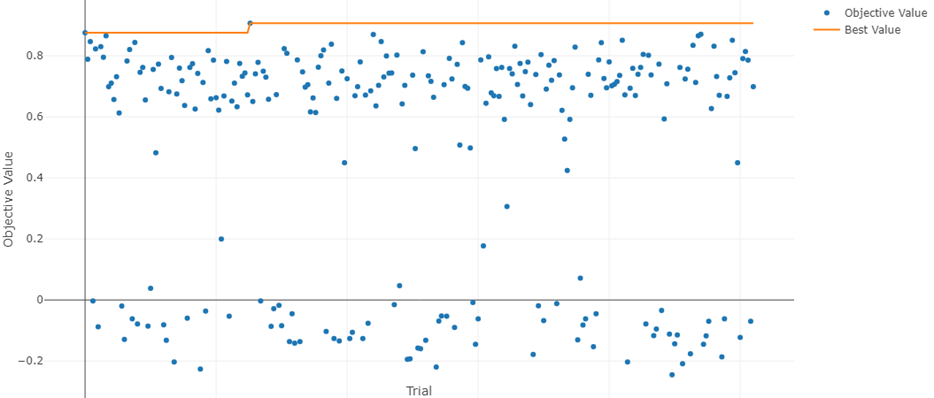
\includegraphics[width=15cm]{figures/figure-4.4.2.png}
% 	\caption[Trials Performance Distribution of RandomSampler - Experiment 4]{Scatter plot of the distribution of the performance of the trials of the RandomSampler in Experiment 4.}
% 	\label{fig:figure-4.4.2}
% \end{figure}
% 
% \begin{figure}[t]
% 	\centering
% 	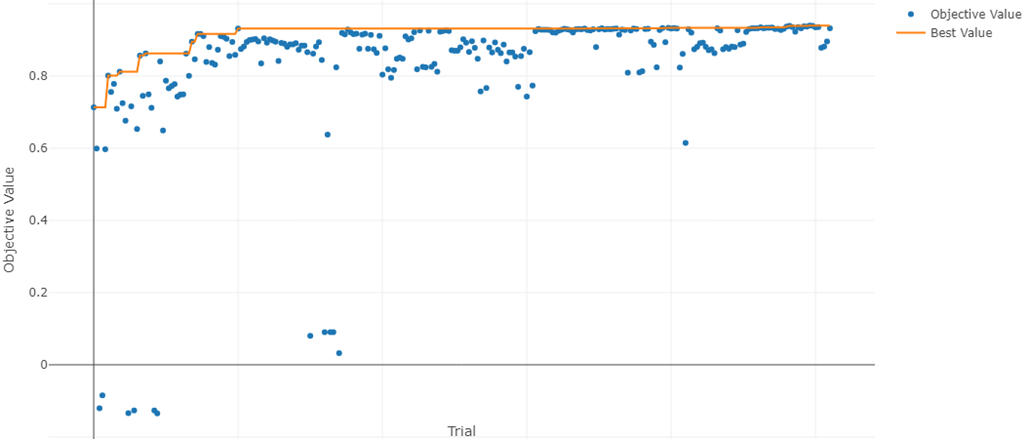
\includegraphics[width=15cm]{figures/figure-4.4.3.png}
% 	\caption[Trials Performance Distribution of TPESampler - Experiment 4]{Scatter plot of the distribution of the performance of the trials of the TPESampler in Experiment 4.}
% 	\label{fig:figure-4.4.3}
% \end{figure}
% 
% \begin{figure}[t]
% 	\centering
% 	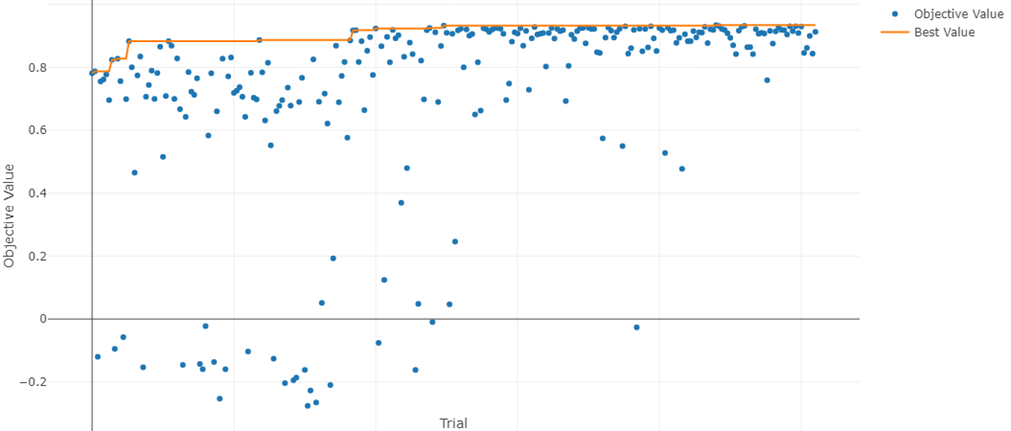
\includegraphics[width=15cm]{figures/figure-4.4.4.png}
% 	\caption[Trials Performance Distribution of PSOSampler - Experiment 4]{Scatter plot of the distribution of the performance of the trials of the PSOSampler in Experiment 4.}
% 	\label{fig:figure-4.4.4}
% \end{figure}
% 

\subsubsection{Analysis of the Hyperparameters Importance}

In this experiment, being all the sub-experiments part of Optuna, it was possible to use Optuna Storage to generate some plots.
\\[0.3cm]All three Samplers generated similar Hyperparameters Importance histograms. In all three, it is evident how the three hyperparameters associated with the layer width are not at the same level of importance, when they should be (Fig.~\ref{fig:figure-4.4.1}). The reason for this is not entirely clear, but it is probably again due to the fact that the problem is very simple, so almost any change in the hyperparameters can lead to a good result, moving away the focus from the importance of the architecture complexity.
\\[0.3cm]The most important hyperparameter appears to be the optimizer; this is probably as a result of the fact that there are only two optimizers, and Adam is almost always better than SGD, therefore making the final score obtain a great advantage.
\begin{figure}[H]
    \begin{minipage}{\textwidth}
        \centering
        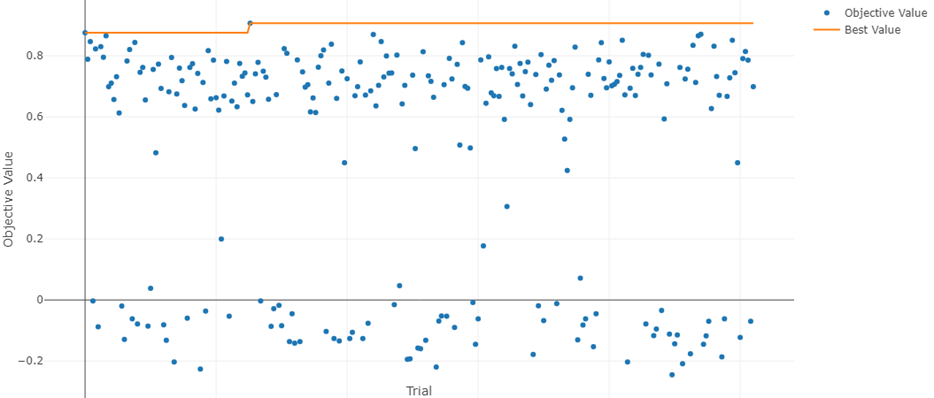
\includegraphics[width=13.8cm]{figures/figure-4.4.2.png}
        \caption[Trials Performance Distribution of RandomSampler - Experiment 4]{Scatter plot of the distribution of the performance of the trials of the RandomSampler in Experiment 4.}
        \label{fig:figure-4.4.2}
    \end{minipage}

    \begin{minipage}{\textwidth}
        \centering
        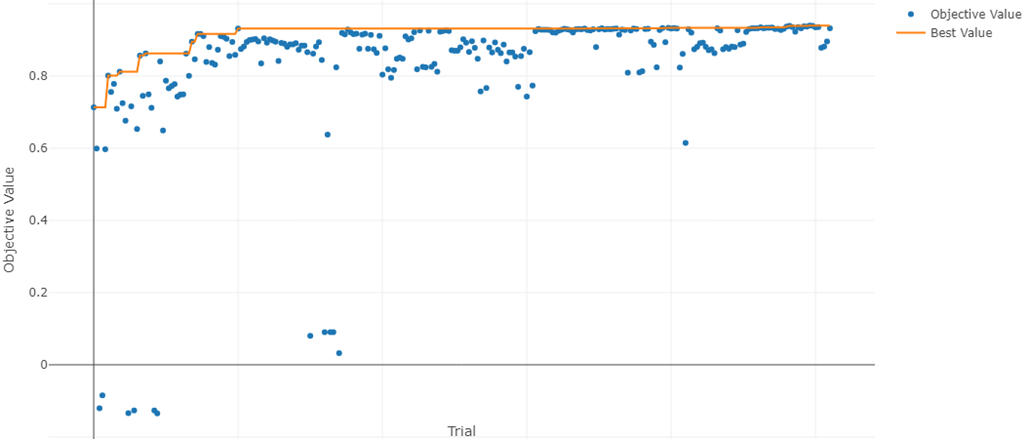
\includegraphics[width=13.8cm]{figures/figure-4.4.3.png}
        \caption[Trials Performance Distribution of TPESampler - Experiment 4]{Scatter plot of the distribution of the performance of the trials of the TPESampler in Experiment 4.}
        \label{fig:figure-4.4.3}
    \end{minipage}

    \begin{minipage}{\textwidth}
        \centering
        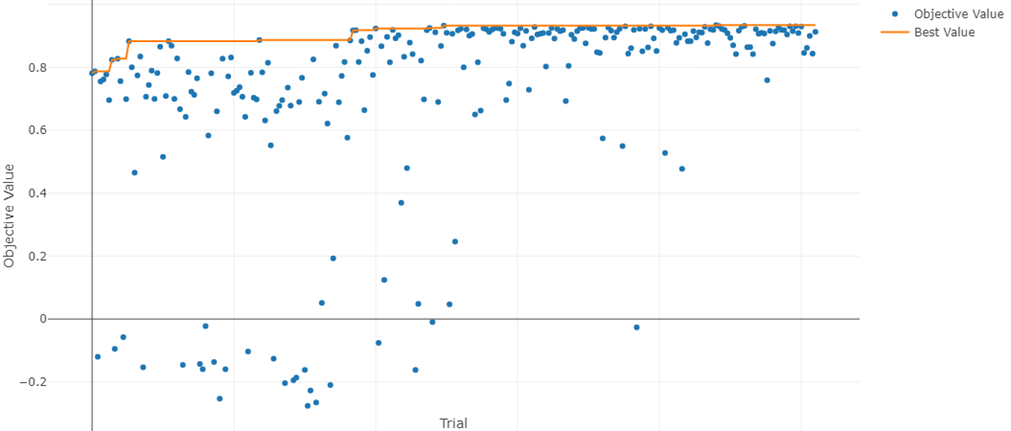
\includegraphics[width=13.8cm]{figures/figure-4.4.4.png}
        \caption[Trials Performance Distribution of PSOSampler - Experiment 4]{Scatter plot of the distribution of the performance of the trials of the PSOSampler in Experiment 4.}
        \label{fig:figure-4.4.4}
    \end{minipage}
\end{figure}
\begin{figure}[t]
	\centering
	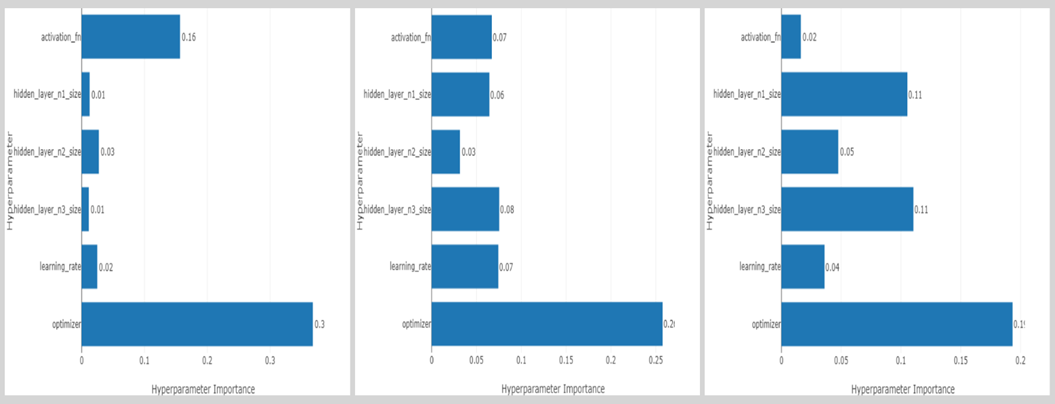
\includegraphics[width=15cm]{figures/figure-4.4.1.png}
	\caption[Hyperparameters Importance Histograms Experiment 4]{Comparison between the generated histograms of the importance of the hyperparameters of Experiment 4. From left to right, Studies of: RandomSampler, TPESampler, PSOSampler.}
	\label{fig:figure-4.4.1}
\end{figure}

\section{Experiment 5 - Hyperparameter Optimization on Weed Map Dataset}

The goal of this experiment is to perform a Hyperparameter Optimization, using the samplers from the previous experiments, for a Weed Mapping problem.
\\[0.3cm]In Drone Vision, Semantic Segmentation is applied to identify immediately and automatically the different categories of “object” inside a cultivated field (crop, terrain, weed). But drones, especially those used for agriculture, do not carry powerful computers able to run complex Neural Networks Models.
\\[0.3cm]Therefore, it is necessary to execute a Hyperparameter Optimization of a NN model for Drone Vision, in order to find a candidate solution that is lightweight but does not lose too much generalization power.
\\[0.3cm]The model utilized for this experiment is Lawin, which is introduced in its relative section in the Methodology chapter (Sec.~\ref{sec:Lawin-3.4.1.2}).
\\[0.3cm]The Dataset of the experiment is Weed Map, a popular dataset for Drone Vision.

\myparagraph{Hardware used for the Experiment:}
The hardware that was utilized to run this experiment is the following:
\begin{itemize}[itemsep=0.1cm]
	\item CPU: AMD EPYC 7V12(Rome) @ 2.45GHz (4-core)
	\item GPU: NVIDIA Tesla T4 (16GB VRAM)
	\item RAM: 28GB
	\item Disk: SSD
	\item OS: Linux (Ubuntu)
\end{itemize}
(This hardware is a Virtual Machine on the Azure ML servers).

\subsection{Weed Map Dataset}

\subsubsection{Introduction to Weed Map Dataset}

The Weed Map Dataset is the dataset for the research “WeedMap: A large-scale semantic weed mapping framework using aerial multispectral imaging and deep neural network for precision farming” \cite{Tesi-2.1}.
\\[0.3cm]Each picture of the Dataset shows an image of a cultivated field, where there can be distinguished Dirt, Weeds and Crops.
\\[0.3cm]The image below (Fig.~\ref{fig:figure-4.5.1}) is an example of one of the images. It is first shown the entire Orthomosaic Map, and then different zoom levels. This highlights the large scale of the image and the difficulty in distinguishing between Crops and Weeds.
\begin{figure}[t]
	\centering
	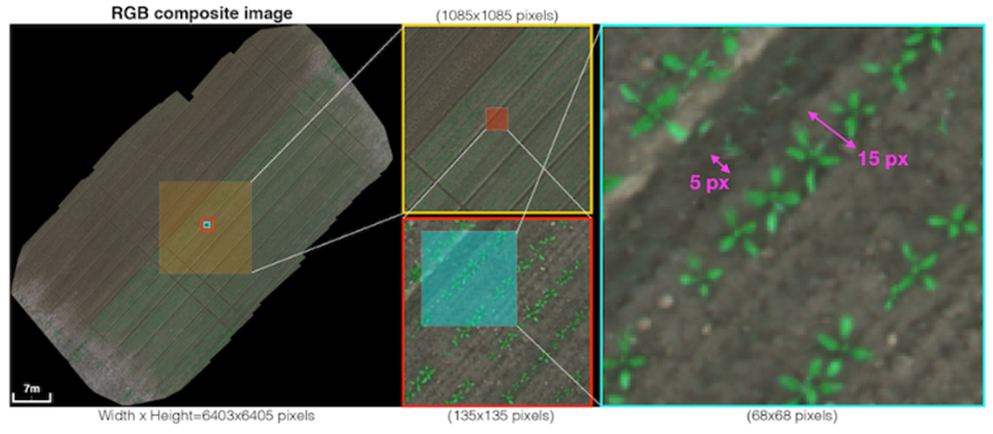
\includegraphics[width=14cm]{figures/figure-4.5.1.png}
	\caption[Example of image in Weed Map Dataset]{Example of image in Weed Map Dataset; with different zoom levels. Source:~\cite{Tesi-2.1}}
	\label{fig:figure-4.5.1}
\end{figure}

\myparagraph{Data Collection:}
The data included in the dataset was collected from aerial images (with Drones) from two different Sugar Beet fields: Eschikon (Switzerland) and Rheinbach (Germany). (Fig.~\ref{fig:figure-4.5.2})
\\[0.3cm]In particular, the utilized Drones are two commercial quadrotor UAVs, equipped with multispectral cameras.
\begin{figure}[t]
	\centering
	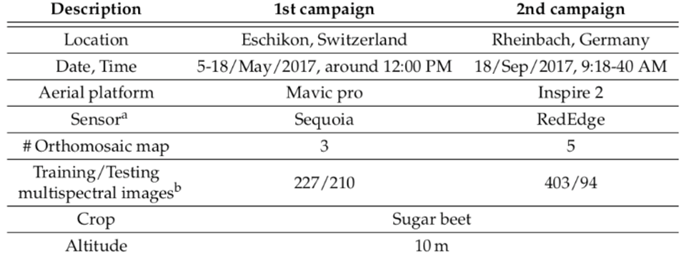
\includegraphics[width=13cm]{figures/figure-4.5.2.png}
	\caption[Information on Campaigns of Weed Map Dataset]{Information on the campaigns of data collection of Weed Map Dataset. Source:~\cite{Tesi-2.1}}
	\label{fig:figure-4.5.2}
\end{figure}

\subsubsection{Structure of Weed Map Dataset}

The full Dataset consist of 129 directories, for a total of 18746 image files. The total weight is 5.36GB.

\myparagraph{Folder Structure:}
There are two main folders, which are Orthomosaic and Tiles.
Orthomosaic contains the full orthomosaic maps.
Tiles contains, for each orthomosaic map, a folder containing images that represent cropped sections of the original orthomosaic map. All cropped sections together form the full map.
\\[0.3cm]Both Orthomosaic and Tiles contain RedEdge and Sequoia subfolders, containing 8 Orthomosaic maps in total (5 RedEdge and 3 Sequoia). (Fig.~\ref{fig:figure-4.5.3})
\\[0.3cm]Each Orthomosaic map stands in a folder indexed from 000 to 007.
\begin{figure}[t]
	\centering
	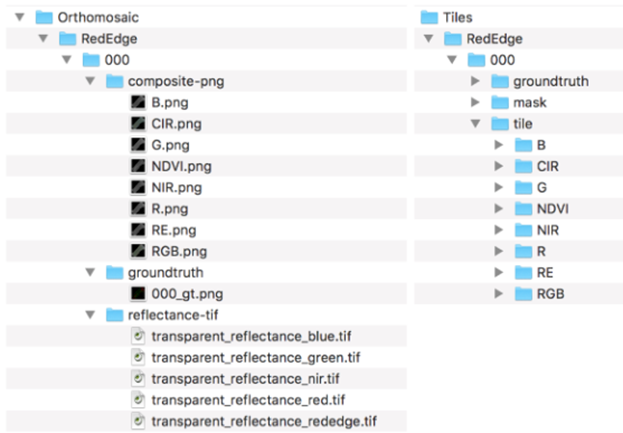
\includegraphics[width=10cm]{figures/figure-4.5.3.png}
	\caption[Folder Structure Weed Map Dataset]{Table showing the folder structure of Weed Map Dataset. Source:~\cite{Tesi-2.1}}
	\label{fig:figure-4.5.3}
\end{figure}

\myparagraph{Groundtruth:}
The Groundtruth images are pictures of the fields where each pixel has been manually labeled. (Fig.~\ref{fig:figure-4.5.4})
Each class is represented in a different colour:
\begin{itemize}[itemsep=0.1cm]
	\item Background (Dirt and part and part of the image which is not the crop field): is Black (code 0)
	\item Crops: is Green (code 1)
	\item Weeds: is Red (code 2)
\end{itemize}
The Groundtruth images are utilized to evaluate the precision of each prediction.
\begin{figure}[t]
	\centering
	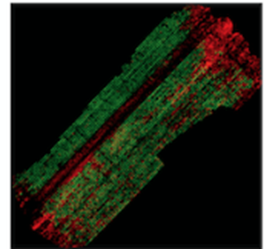
\includegraphics[width=5cm]{figures/figure-4.5.4.png}
	\caption[Example of GroundTruth in Weed Map Dataset]{Example of GroundTruth image in Weed Map Dataset. Source:~\cite{Tesi-2.1}}
	\label{fig:figure-4.5.4}
\end{figure}

\subsection{Preparation of the Experiment}

This experiment is partially different from the previous experiments. All studies continue to be initialized with the “wrapping”.
\\[0.3cm]The architectures with which to initialize the NN are no longer built inside the objective function, and thus need to be defined earlier. The architectures subject of this experiment are defined in the same article in which the original experiment of Weed Mapping was proposed \cite{WeedMap-PaperThesis}. During the experiment, those architectures will be referenced as “backbone”.
\\[0.3cm]The Weed Map dataset was loaded using the pre-defined function mentioned in the related section of the Methodology chapter (Sec.~\ref{sec:Lawin-3.4.1.2}). The utilized version of Weed Map Dataset is not the original version, but is a pre-processed one (the same as \cite{WeedMap-PaperThesis}).

\subsubsection{Setup of the Studies}

% \myparagraph{Initialize the Studies:}
The samplers of Optuna used to perform three different HPOs, are the following: \texttt{RandomSampler}, \texttt{TPESampler}, \texttt{PSOSampler}.
For each of the samplers, an Optuna \texttt{Study} is created. All the standard samplers are initialized with their default input values. The \texttt{PSOSampler} is initialized with two values, \texttt{num\_particles} and \texttt{max\_generations}.
\\[0.3cm]The Pruning mechanism used is the Median Pruning algorithm. It is applied through the \texttt{MedianPruner} object of Optuna, whose values for initialization are below.

\subsubsection{Setup of the Objective Function}

% \myparagraph{Objective Function:}
The objective function, as always, is the same for each Study. The structure of the objective function is the same as in the last experiments.
\\[0.3cm]It is important to note one difference, which is the metric to follow. Although all four metrics are always computed, in this experiment the F1-Score will be the main metric, differently from the previous experiments where it was Accuracy.
\\[0.3cm]The initialization hyperparameters of the loss function, \texttt{Focal}, were fixed. Their chosen values are: \texttt{gamma} = 2, \texttt{weights} = [0.06, 1, 1.7].
% 
% \myparagraph{Search Space of Hyperparameters:}
\\[0.3cm]The Hyperparameters declared in the objective function, which form the Search Space of the Study, for this experiment were the following (Tab.~\ref{tab:table-4.5.1}).
\begin{table}[ht!]
	\center
	\setlength{\tabcolsep}{0.5cm}
	\caption[Search Space of Experiment 5]{Search Space of Experiment 5: list of hyperparameters and their values ranges, with the step. Where Step is $\sim$ if the range is continuous.}
	\begin{tabular}{@{}lcc@{}}
		\toprule
		\textbf{Hyperparamter} & \textbf{Range}                             & \textbf{Step} \\ \midrule
		Backbone               & \{MiT-B0, MiT-LD, MiT-L0, MiT-L1, MiT-L2\} & -             \\[0.1cm]
		Learning Rate          & {[}$10^{-4}$, $10^{-2}${]}                 & $\sim$        \\[0.1cm]
		Optimizer              & \{SGD, Adam\}                              & -             \\ \bottomrule
	\end{tabular}
	\label{tab:table-4.5.1}
\end{table}
% 
% \myparagraph{Optimizing Process Parameters:}
\\[0.3cm]Other parameters, related to the Optimization process, basically hyperparameters of the HPO process itself (could be called “Hyper-Hyperparamters”), which were used are the following (Tab.~\ref{tab:table-4.5.2}).
\begin{table}[ht!]
	\center
	\setlength{\tabcolsep}{0.5cm}
	\caption[Optimization External Parameters of Experiment 5]{External optimization parameters of Experiment 5, basically hyperparameters of the optimization process, with their values.}
	\begin{tabular}{@{}llc@{}}
		\toprule
		\textbf{Group}                & \textbf{Parameter} & \textbf{Value} \\ \midrule
		Regularizer                   & labda              & 0.4            \\[0.1cm]
		EarlyStopper                  & patience           & 15             \\[0.2cm]
		\multirow{2}{*}{PSOSampler}   & num\_particles     & 32             \\[0.1cm]
									  & max\_generations   & 8              \\[0.2cm]
		\multirow{4}{*}{MedianPruner} & n\_startup\_trials & 2              \\[0.1cm]
									  & n\_warmup\_steps   & 20             \\[0.1cm]
									  & interval\_steps    & 20             \\[0.1cm]
									  & n\_min\_trials     & 4              \\ \bottomrule
	\end{tabular}
	\label{tab:table-4.5.2}
\end{table}

\subsection{Execution of the Experiment}

The execution of each Study is handled by an OptunaRunner object for Optuna, which at the end of the optimization process saves the results on a csv file.
\\[0.3cm]The number of Trials executed for each Study was 64.

\subsubsection{Score Results}

The best score achieved by the \texttt{RandomSampler} is 70\%; the top trials have as backbone MiT-L1 and MiT-L2; F1-Score of the best trials is around 69\%-74\%.
\\[0.3cm]The best score achieved by the \texttt{TPESampler} is 74.4\%; the top trials have as backbone MiT-L2; the F1-Score of the best trials is around 70\%-77\%.
\\[0.3cm]The best score achieved by the \texttt{PSOSampler} is 67\%; the top trials have as backbone MiT-L1; the F1-Score of the best trials is around 68\%-75\%.
\\[0.3cm]For all three samplers, the best trials in terms of F1-Score have as backbones MiT-B0 and MiT-LD.

\subsubsection{Hyperparameters Results}

The Hyperparameters Importance graph is shown in the figure (Fig.~\ref{fig:figure-4.5.5}), which is the one generated from \texttt{TPESampler}, being the Study with the best results, even though also the other two studies generated very similar results.
\begin{figure}[t]
	\centering
	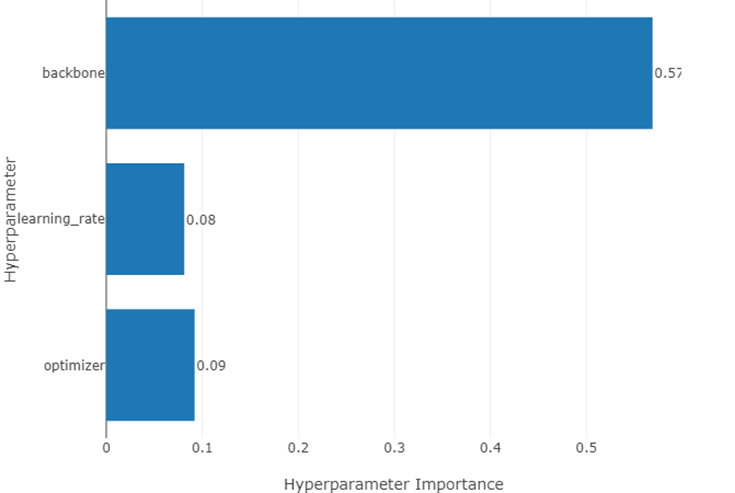
\includegraphics[width=13cm]{figures/figure-4.5.5.png}
	\caption[Hyperparameters Importance Histogram Experiment 5]{Histogram of the importance of the hyperparameters of Experiment 5, generated by the Study of TPESampler.}
	\label{fig:figure-4.5.5}
\end{figure}
\\[0.3cm]The best candidate solution, and thus the best found hyperparameters are:
\begin{itemize}[itemsep=0.1cm]
    \item Backbone = MiT-L2
    \item Learning Rate = 0.002
    \item Optimizer = Adam
\end{itemize}

\subsection{Discussion of the Results}

The results the of experiment allowed to find a valid hyperparameters' configuration that solves the initial problem.
In fact, the proposed solution, uses the most lightweight among all the Backbones, creating the most lightweight Neural Network for the Drone Vision problem possible.

\subsubsection{Analysis of the Performance of the Samplers}

The \texttt{RandomSampler} worked as usual, there does not seem to be any problem with its functioning. The \texttt{TPESampler} found good solutions, therefore, it could be argued that it is working as supposed. The \texttt{PSOSampler} on the other hand, showed results beneath expectations.
\\[0.3cm]The reason \texttt{PSOSampler} underperformed in this particular experiment, is because of the way pruning influences the sampler in more complex problems like this experiment.
Differently from \texttt{TPESampler}, \texttt{PSOSampler} also considers the pruned trials when updating its local and global optimum positions. Differently from previous experiments, in this one the score of a pruned trial is often very high, sometimes also between the highest scores (this is because there is a lot of difference between Validation Set and Test Set evaluations, and the latter is performed only if a trial is not pruned). This confuses, or better, misleads the particles of PSO, resulting in the algorithm finding low quality results.
\\[0.3cm]This is easily fixable, but given that \texttt{TPESampler} already found the best results, and the cost of the execution of a single Study is outrageously high, this remains a recommendation for the future.

\subsubsection{Analysis of the Quality of Results}

The considered results for this analysis are the ones from the \texttt{TPESampler}, as it was the sub-experiment with the best results among all samplers.
\\[0.3cm]The best solutions all have in common the same Backbone, which is MiT-L2. This is the lightest Backbone among the proposed ones.
Tested singularly with already known good hyperparameters, the MiT-B0 and MiT-LD, which are deeper, more complex architectures, have obtained results around 76\% of F1-Score on the Test Set.
The best solution obtained by the \texttt{TPESampler} with the MiT-L2 architecture obtained a F1-Score of 74.4\%, which is only 1.6\% apart from the best architecture.
\\[0.3cm]Therefore, this experiment could be considered a success, as the architecture of the Neural Network was heavily simplified from a total of 1024 neurons to 64 (MiT-B0 and MiT-L2 respectively), losing only 1.6\% from the performance.




